%!TEX root = ./main.tex

\section{Online \emph{linear} covering with multiple experts}	\label{sec:covering}

\subsection{Benchmark relaxation for the algorithm}

Our first proposed algorithm solves online linear covering problems by creating linear combinations of the solutions proposed by $K$ experts in an online manner.
Recall that we evaluate the performance of our algorithm with the \texttt{LIN-COMB} benchmark (formalized on \cref{fig:benchmark}), which consists of the best linear combination of the experts' solution at each time step.

Since our \texttt{LIN-COMB} benchmark is a linear combination of the experts' solutions, the equality $ \sum_{k=1}^{K} w_{k}^{t} = 1$ must hold, where $w_{k}^{t} \geq 0$ is the weight assigned to expert $k$ (where $1 \leq k \leq K$) at time $t$. In the following, we formulate a relaxed version of the \texttt{LIN-COMB} formulation, where
$\sum_{k=1}^{K} w_{k}^{t} \geq 1$. Additionally, the relaxed formulation enables us to avoid the (online) hard constraint requiring $w_{k}^{t} s_{i,k}^{t} \geq w_{k}^{t-1} s_{i,k}^{t-1}$ to hold, and instead, we introduce a new variable, $y_{i}^{t}$, to represent the increase of $x_{i}^{t}$ compared to $x_{i}^{t-1}$. When $w_{k}^{t} s_{i,k}^{t} < w_{k}^{t-1} s_{i,k}^{t-1}$ during the execution, we set the contribution of $i$ at time $t$ to be 0, and therefore, $y_{i}^{t} = 0$.
The relaxed formulation is visible on Figure~\ref{fig:relaxation}.

Due to the relaxed constraint, the optimal solution of the relaxed linear program is a lower bound of our \texttt{LIN-COMB} benchmark. The dual of the relaxation is displayed on Figure~\ref{fig:dual}.


\begin{figure}[ht]
	\begin{mdframed}
		\begin{align*}
			&& \min \sum_{t = 1}^{T} \sum_{i=1}^{n} & c_i y_i^t \\
			%
			(\alpha^{t}) \qquad && \sum_{k=1}^{K} w_{k}^{t} & \geq 1  & \forall\ t \\
			%
			(\beta_{i}^{t}) \qquad && \sum_{k=1}^{K} \left(w_{k}^{t} s_{i,k}^{t} - w_{k}^{t-1} s_{i,k}^{t-1} \right) &\leq y_i^t  &\forall\ i,t\\
		%
			&& w_{k}^{t},\ y_{i}^{t} & \ge 0 & \forall\ i,t,k
		\end{align*}
		%\vspace{5pt}
	\end{mdframed}
	\caption{Formulation of the relaxation of the \texttt{LIN-COMB} benchmark}
	\label{fig:relaxation}
\end{figure}

\begin{figure}[ht]
	\begin{mdframed}
		\begin{align*}
			&& \max \sum_{t=1}^{T} & \alpha^{t} \\
		%
			(w_{k}^{t}) \qquad && \alpha^{t} + \sum_{i=1}^{n} s_{i,k}^{t} ( \beta_{i}^{t+1} - \beta_{i}^{t})   &\leq 0  &\forall\ k,t\\
		%
			(y_{i}^{t}) \qquad && \beta_{i}^{t}   &\leq c_{i}  &\forall\ i,t \\
		%
			&& \alpha_{i}^{t},\ \beta_{i}^{t} & \ge 0 & \forall\ i,t
		\end{align*}
		%\vspace{5pt}
	\end{mdframed}
	\caption{Dual formulation of the relaxation of the \texttt{LIN-COMB} benchmark}
	\label{fig:dual}
\end{figure}


According to the theorem of weak duality, any feasible solution of the dual program lower bounds any feasible solution of the primal program, and therefore, any feasible dual solution also lower bounds our \texttt{LIN-COMB} benchmark. Following the chain of lower bounds, our approach to design a competitive algorithm is as follows. At every time step $t$, we build solutions for all $x_{i}^{t}$ together with the solutions for the dual problem $(\alpha^{t}, \beta_{i}^{t})$. Then, we bound the cost of the algorithm to that of the dual. It is important to emphasize that the designed solution for every $x_{i}^{t}$ must be feasible to the covering constraints, but it may \emph{not necessarily} be a linear combination of the experts' solutions.

\subsection{Algorithm description} \label{sec:algo}

\paragraph{Preprocessing.}
Recall that by our assumptions, the experts' solutions are always feasible and non-decreasing. At the arrival of the $t^{\text{th}}$ constraint, expert $k$ (where $1 \leq k \leq K$) provides a feasible solution $s_{k}^{t} = (s_{i,k}^{t})_{i=1}^{n}$, such that $s_{i,k}^{t} \ge s_{i,k}^{t'}$ for all $t' \le t$ and all $i$ where $1 \le i \le n$. These assumptions do not exclude the possibility for the experts to provide malicious solutions that instruct the algorithm to use an unnecessarily large amount of resources.
To regardless maintain online solutions, we do \emph{not} expect the experts' solutions to be always tight (a difference compared to the assumptions in \cite{AnandGe22:Online-Algorithms}).
%Either the solutions come from an offline method and guarantee tightness as in \cite{BamasMaggoriSvensson20:primal-dual-method}, or the solutions are constructed online by the experts and do not guarantee tightness.
(In Appendix~\ref{appix-tight-solutions}
we show an example that tight solutions cannot be maintained in an online manner.)


To circumvent the issue of malicious suggestions, we preprocess the experts' solutions at each iteration. During the preprocessing, every solution $s_k^t$ is scaled down to make it as tight as possible on the $t^{\text{th}}$ constraint, while always maintaining $s_{i,k}^{t} \geq s_{i,k}^{t-1}$ for all $i$. Additionally, after the down-scaling, we create an auxiliary solution $\hat{s}_k^t$ that is tight for the $t^{\text{th}}$ constraint. This auxiliary solution is useful for our algorithm and its analysis, but it does not directly participate in forming the actual solution. (Our algorithm only sets the weights of the experts and does not change the experts' solutions.) The auxiliary solution $\hat{s}_k^t$ is created with the following procedure.

After the down-scaling, do the following for each expert $k$.
\begin{compactenum}
	\item If $(s_{i,k}^{t})_{i=1}^{n}$ is tight on the $t^{\text{th}}$ constraint, then set $\hat{s}_{i,k}^{t} \gets s_{i,k}^{t}$  for every $i$.
	\item Let $\hat{s}_{i,k}^{t-1}$ be the auxiliary solution of expert $k$ at time $t-1$, meaning that, $\sum_{i=1}^{n} a_{i}^{t-1} \hat{s}_{i,k}^{t-1} = 1$. Given $I := \{i: s_{i,k}^{t} > \hat{s}_{i,k}^{t-1} \cdot \frac{a_{i}^{t-1}}{a_{i}^{t}} \}$, we set $\hat{s}_{i,k}^{t} \gets s_{i,k}^{t}$ if $i \notin I$
	and set $\hat{s}_{i,k}^{t}$ to be some value in $[\hat{s}_{i,k}^{t-1} \cdot \frac{a_{i}^{t-1}}{a_{i}^{t}}, s_{i,k}^{t}]$ if $i \in I$, s.t. the solution $\hat{s}_{i,k}^{t}$
	becomes tight on the $t^{\text{th}}$ constraint.
%	\item Otherwise, let $t' < t$ be the last constraint where expert $k$ provides a solution which is tight.
%	We define a set $I := \{i: s_{i,k}^{t} > s_{i,k}^{t'} \cdot \frac{a_{i}^{t'}}{a_{i}^{t}} \}$. Then, set $\hat{s}_{i,k}^{t} \gets s_{i,k}^{t}$ for $i \notin I$
%	and set $\hat{s}_{i,k}^{t}$ to be some value in $[s_{i,k}^{t'} \cdot \frac{a_{i}^{t'}}{a_{i}^{t}}, s_{i,k}^{t}]$ if $i \in I$, such that the solution $\hat{s}_{i,k}^{t}$
%	becomes tight on the $t^{\text{th}}$ constraint.
\end{compactenum}
%
\begin{lemma}
Following the preprocessing procedure, we can always obtain the solutions $\hat{s}_{i,k}^{t}$ such that
$\hat{s}_{i,k}^{t} \leq s_{i,k}^{t}$ and $\sum_{i=1}^{n} a_{i}^{t} \hat{s}_{i,k}^{t} = 1$.
\end{lemma}
%
\begin{proof}
Let us fix an expert $k$. We prove the lemma by induction. At time step $t=1$, we can always scale down the solution $s_{i,k}^{1} \geq 0$ such that the first constraint becomes tight.
Assume that the lemma holds until $t-1$, so $\sum_{i=1}^{n} a_{i}^{t-1} \hat{s}_{i,k}^{t-1} = 1$ and $\hat{s}_{i,k}^{t-1} \leq s_{i,k}^{t-1}$.
Consider time $t$. If after the down-scaling (during the first prepocessing step) the $t^{\text{th}}$ constraint becomes tight, then we are done. Otherwise, we have
	%
	\begin{align*}
		1 &< \sum_{i=1}^{n} a_{i}^{t} s_{i,k}^{t} = \sum_{i \in I} a_{i}^{t} s_{i,k}^{t} + \sum_{i \notin I} a_{i}^{t} s_{i,k}^{t}  & \\
		%
		& & \text{and} \\
		%
		1 &= \sum_{i=1}^{n} a_{i}^{t-1} \hat{s}_{i,k}^{t-1} =  \sum_{i = 1}^{n} a_{i}^{t} \biggl( \hat{s}_{i,k}^{t-1} \cdot \frac{a_{i}^{t-1}}{a_{i}^{t}} \biggr) & \\
		&\geq  \sum_{i \in I} a_{i}^{t} \biggl( \hat{s}_{i,k}^{t-1} \cdot \frac{a_{i}^{t-1}}{a_{i}^{t}} \biggr)
		+ \sum_{i \notin I} a_{i}^{t} s_{i,k}^{t} &
	\end{align*}
	%
	Hence, there exists $\hat{s}_{i,k}^{t} \in \bigl[ \hat{s}_{i,k}^{t-1} \cdot \frac{a_{i}^{t-1}}{a_{i}^{t}}, s_{i,k}^{t} \bigr]$ for every $i$, where $1 \leq i \leq n$, such that $\sum_{i=1}^{n} a_{i}^{t} \hat{s}_{i,k}^{t} = 1$.
\end{proof}

\noindent \paragraph{Remark.} Our proposed algorithm solves a convex program at each time step to set the current value of the variables. The convex program's objective uses a shifted entropy function as a convex regularizer. To avoid a possible division by $0$ while solving the convex program, we use a dummy expert. This expert sets initially each variable to some small value, then follows the greedy heuristic and resolves the problem at each arriving constraint. The presence of this dummy expert only changes the competitive ratio from $O(\log(K))$ to $O(\log(K + 1))$. However, we display all other occurrences of the competitive ratio as $O(\log(K))$ for simplicity. Additionally, at time $0$ (when no constraints have arrived yet), every expert's suggestion is $0$ for every variable, but the average of the suggestions is $1$.

\clearpage

\paragraph{Algorithm.}

At the arrival of the $t^{\text{th}}$ constraint,
\begin{compactenum}
	\item solve the following convex program and set $w^t$ to be the obtained optimal solution
%
\begin{align*}
&& \min_{w} \biggl\{\sum_{i=1}^{n} c_{i}  \biggl[  \biggl(\sum_{k=1}^{K} s_{i,k}^{t} w_{i,k}  + \delta_{i}^{t} \biggr) &
					 \ln \left( \frac{\sum_{k=1}^{K} s_{i,k}^{t} w_{i,k}  + \delta_{i}^{t}}{ \sum_{k=1}^{K}  s_{i,k}^{t-1}w_{i,k}^{t-1}  + \delta_{i}^{t-1}}  \right)
					 		- \sum_{k=1}^{K}  s_{i,k}^{t} w_{i,k} \biggr] \biggr\} \\
%\end{align*}
%%
%\noindent subject to:
%%
%\begin{align*}
    (\gamma^{t})  && \sum_{i=1}^{n} a_{i}^{t} \biggl( \sum_{k=1}^{K}  \hat{s}_{i,k}^{t} w_{i,k} \biggr) &\geq 1 \qquad \forall\ t\\
%
    (\lambda_{i}) && \sum_{k=1}^{K}  w_{i,k} &\geq 1 \qquad \forall\ i\\
%
    (\mu_{i}^{t}) && \sum_{k=1}^{K} s_{i,k}^{t} w_{i,k} &\geq 0 \qquad \forall\ i,t
\end{align*}
%
where $\delta_{i}^{t} = \frac{1}{K} \sum_{k} s_{i,k}^{t}$.
%and recall that we set $\rho = \max_{i} \max_{t',t''} \left\{\frac{\sum_{k=1}^{K} s_{i,k}^{t'}}{\sum_{k=1}^{K} s_{i,k}^{t''}} : \sum_{k=1}^{K} s_{i,k}^{t''} > 0 \right\}$.
Note that in this program, we use the auxiliary solution $\hat{s}_{i,k}^{t}$ in the first constraint. For every $i$ where $s_{i,k}^{t} = 0$ for all $k$, the term related to $i$ is not included in the objective function of the convex program.
(We can set $w_{i,k} = 0$ for all $k$ beforehand.)
	%
	\item For all $i$, if $\sum_{k} w_{i,k}^{t} s_{i,k}^{t} > x_{i}^{t-1}$ then set $x_{i}^{t} \gets \sum_{k} w_{i,k}^{t} s_{i,k}^{t}$;
otherwise set $x_{i}^{t} \gets x_{i}^{t-1}$.
\end{compactenum}

\medskip

\subsection{Performance Analysis}
As $w^{t}$ is the optimal solution of the convex program and ($\gamma^t,\ \lambda_{i},\ \mu_{i}^{t}$) is the optimal solution of its dual, the following Karush-Kuhn-Tucker (KKT) and complementary slackness conditions hold.

\begin{align*}
   \biggl[ \sum_{i=1}^{n} a_{i}^{t} \biggl( \sum_{k=1}^{K}  \hat{s}_{i,k}^{t} w_{i,k}^{t} \biggr) - 1 \biggr] \gamma^{t} &= 0 \qquad \forall\ t \\
   \biggl[ \sum_{k=1}^{K}  w_{i,k}^{t}  - 1 \biggr] \lambda_{i} &= 0 \qquad \forall\ i, t \\
   \biggl[ \sum_{k=1}^{K}  s_{i,k}^{t} w_{i,k}^{t} \biggr] \mu_{i}^{t} &= 0 \qquad \forall\ i, t \\
%
 c_{i} s_{i,k}^{t} \ln \left( \frac{\sum_{k=1}^{K} s_{i,k}^{t} w_{i,k}^{t} + \delta_{i}^{t}}{\sum_{k=1}^{K}  s_{i,k}^{t-1}w_{i,k}^{t-1}  + \delta_{i}^{t-1}} \right)
    	- a_{i}^{t} \hat{s}_{i,k}^{t} \gamma^{t} - \lambda_{i} - s_{i,k}^{t} \mu_{i}^{t} &= 0	\qquad \forall\ i,k,t \\
	%
	\gamma^{t}, \lambda_{i}, \mu_{i}^{t} &\geq 0 \qquad \forall\ i, t
\end{align*}

Moreover, if $\sum_{k} w_{i,k}^{t} s_{i,k}^{t} > 0$, meaning that $\mu_{i}^{t} = 0$, then
\begin{align}	\label{eq:KKT1}
   c_{i} s_{i,k}^{t} \ln \left( \frac{\sum_{k=1}^{K} s_{i,k}^{t} w_{i,k}^{t}  + \delta_{i}^{t}}{\sum_{k=1}^{K}  s_{i,k}^{t-1}w_{i,k}^{t-1}  + \delta_{i}^{t-1}} \right)
    	- a_{i}^{t} \hat{s}_{i,k}^{t} \gamma^{t} - \lambda_{i} = 0
\end{align}

\clearpage

\paragraph{Dual variables and feasibility.} We set the dual variables of the linear program relaxation of our \texttt{LIN-COMB} benchmark based on the dual variables of the convex program used inside the algorithm. The dual formulation is visible on \cref{fig:dual}.
%
\begin{align*}
    \alpha^{t} &= \frac{1}{\ln(K\rho)}  \biggl( \gamma^{t} + \sum_{i=1}^{n} \lambda_{i} \biggr), \\
    \beta_{i}^{t} &= \frac{1}{\ln(K\rho)} c_i \ln \left(\frac{ (1 + 1/K) \cdot \max_{t'} \sum_{k=1}^{K} s_{i,k}^{t'}}{\sum_{k=1}^{K}  s_{i,k}^{t-1} w_{i,k}^{t-1} + \delta_{i}^{t-1}}\right)
\end{align*}
%
where recall that $\rho = \max_{i, t',t''} \left\{\frac{\sum_{k=1}^{K} s_{i,k}^{t'}}{\sum_{k=1}^{K} s_{i,k}^{t''}} : \sum_{k=1}^{K} s_{i,k}^{t''} > 0 \right\}$.

\begin{lemma} \label{lem:covering-feasibility}
The $x_{i}^{t}$ solutions set by the algorithm for the original covering problem and the dual variables $(\alpha^{t}, \beta_{i}^{t})$ of the \texttt{LIN-COMB} benchmark's linear program relaxation are feasible.
\end{lemma}
%
\begin{proof}
We first prove that the $x_{i}^{t}$ variables satisfy the covering constraints by induction. At time 0, no constraint has been released yet, and every variable is set to 0. This all-zero solution is feasible. Let us assume that the algorithm provides feasible solutions up to time $t-1$. At time $t$, the algorithm maintains the inequality $x_{i}^{t} \geq x_{i}^{t-1}$, so all constraints $t'$ where $t' < t$ are satisfied. Besides, $x_{i}^{t}$ is always at least
$\sum_{k} w_{i,k}^{t} s_{i,k}^{t}$, which is larger than $\sum_{k} w_{i,k}^{t} \hat{s}_{i,k}^{t}$ since $s_{i,k}^{t} \geq \hat{s}_{i,k}^{t}$
for all $i,k$ due to the preprocessing step. Hence, the constraint $t$ is also satisfied. Formally,
$$
\sum_{i=1}^{n} a_{i}^{t} x_{i}^{t}  \geq \sum_{i=1}^{n} a_{i}^{t} \biggl( \sum_{k=1}^{K} w_{i,k}^{t}  \hat{s}_{i,k}^{t} \biggr) \geq 1.
$$

In the remaining part of the proof, we show the feasibility of $\alpha^{t}$ and every $\beta_{i}^{t}$.
Since $ \gamma^{t} \geq 0$ and $\lambda_{i} \geq 0$ for all $i$ and $t$, we get that $\alpha^{t} \geq 0$.
When we set $\beta_{i}^{t}$, the nominator of the logarithm term is always larger than the denominator, and it is smaller than $(K\rho)$-times the denominator. Consequently, $0 \leq \beta_{i}^{t} \leq c_{i}$. Furthermore,
%
\begin{align*}
    \beta_{i}^{t+1} - \beta_{i}^{t}
    	&= - \frac{1}{\ln(K\rho)} c_i \ln \left( \frac{\sum_{k=1}^{K}  s_{i,k}^{t} w_{i,k}^{t} + \delta_{i}^{t}}{\sum_{k=1}^{K}  s_{i,k}^{t-1}w_{i,k}^{t-1} + \delta_{i}^{t-1}} \right).
\end{align*}
%
Since $\sum_{i} a_{i}^{t} \hat{s}_{i,k}^{t} = 1$, using the KKT conditions, we get:
\begin{align*}
\alpha^{t} + \sum_{i=1}^{n} s_{ik}^{t} \left(\beta_{i}^{t+1} - \beta_{i}^{t}\right)
&= \frac{1}{\ln(K\rho)} \biggl( \gamma^{t} + \sum_{i=1}^{n} \lambda_{i} \biggr)
	- \frac{1}{\ln(K\rho)}  \sum_{i=1}^{n} s_{i,k}^{t} c_i \ln \left( \frac{\sum_{k=1}^{K}  s_{i,k}^{t} w_{i,k}^{t} + \delta_{i}^{t}}{\sum_{k=1}^{K}  s_{i,k}^{t-1}w_{i,k}^{t-1} + \delta_{i}^{t-1}} \right) \\
%
&= \frac{1}{\ln(K\rho)} \biggl[ \gamma^{t} + \sum_{i=1}^{n} \lambda_{i} - \sum_{i=1}^{n} \left( a_{i}^{t} \hat{s}_{i,k}^{t} \gamma^{t} + \lambda_{i} + s_{i,k}^{t} \mu_{i}^{t} \right) \biggr] \\
%
&\leq 0
\end{align*}
\end{proof}

\clearpage

\begin{theorem} \label{covering-theorem}
The algorithm is $O(\ln(K \rho))$-competitive with the \texttt{LIN-COMB} benchmark.
\end{theorem}
%
\begin{proof} \cref{lem:covering-feasibility} proved that our algorithm creates feasible solutions for the dual problem of the \texttt{LIN-COMB} benchmark's relaxation and for the original covering problem. We show that the algorithm's solution increases the primal objective value of the original covering problem by at most $O(\ln(K \rho))$ times the value of the relaxation's dual solution, which serves as the lower bound on the \texttt{LIN-COMB} benchmark (the best linear combination of the experts' solutions).
\begin{align}
	 \sum_{i=1}^{n} &c_{i} (x_{i}^{t} - x_{i}^{t-1})
		= \sum_{i: x_{i}^{t} > x_{i}^{t-1}} c_{i}(x_{i}^{t} - x_{i}^{t-1}) &&  \notag \\
		%
		&\leq \sum_{i: x_{i}^{t} > x_{i}^{t-1}} c_{i}(x_{i}^{t} + \delta_{i}^{t}) \ln \left(\frac{x_{i}^{t} + \delta_{i}^{t}}{x_{i}^{t-1} + \delta_{i}^{t}}\right) \\
		%
		&\leq \sum_{i: x_{i}^{t} > x_{i}^{t-1}} c_{i} (x_{i}^{t} + \delta_{i}^{t}) \ln \left(\frac{x_{i}^{t} + \delta_{i}^{t}}{x_{i}^{t-1} + \delta_{i}^{t-1}}\right) \\
		%
		&= \sum_{i: x_{i}^{t} > x_{i}^{t-1}} c_{i} \left[ \left(\sum_{k=1}^{K}  s_{i,k}^{t} w_{i,k}^{t} + \frac{1}{K} \sum_{k=1}^{K} s_{i,k}^{t} \right)
			\ln \left(\frac{ \sum_{k=1}^{K}  s_{i,k}^{t} w_{i,k}^{t} + \delta_{i}^{t}}{x_{i}^{t-1} + \delta_{i}^{t-1}}  \right) \right] \\
%
&\leq \sum_{i: x_{i}^{t} > x_{i}^{t-1}} c_{i} \left[ \left(\sum_{k=1}^{K}  s_{i,k}^{t} w_{i,k}^{t} + \frac{1}{K} \sum_{k=1}^{K} s_{i,k}^{t} \right)
			\ln \left(\frac{ \sum_{k=1}^{K}  s_{i,k}^{t} w_{i,k}^{t} + \delta_{i}^{t}}{\sum_{k=1}^{K}  s_{i,k}^{t-1} w_{i,k}^{t-1} + \delta_{i}^{t-1}}  \right) \right]\\
%
	&= \sum_{i: x_{i}^{t} > x_{i}^{t-1}} \sum_{k=1}^{K} (w_{i,k}^{t} + 1/K) c_{i} s_{i,k}^{t}
				\ln \left(\frac{ \sum_{k=1}^{K} s_{i,k}^{t} w_{i,k}^{t}  + \delta_{i}^{t}}{\sum_{k=1}^{K}  s_{i,k}^{t-1} w_{i,k}^{t-1}  + \delta_{i}^{t-1}}  \right) \notag \\
%
%\end{align}
%%
%\begin{align}
%
&=  \sum_{i: x_{i}^{t} > x_{i}^{t-1}} \sum_{k=1}^{K} (w_{i,k}^{t} + 1/K) \biggl( a_{i}^{t} \hat{s}_{i,k}^{t} \gamma^t + \lambda_{i} \biggr) \\
%
%
&\leq \sum_{i=1}^{n} \sum_{k=1}^{K} (w_{i,k}^{t} + 1/K) \biggl( a_{i}^{t} \hat{s}_{i,k}^{t} \gamma^t + \lambda_{i} \biggr) \notag \\
%
&= \sum_{i=1}^{n} a_{i}^{t} \biggl(\sum_{k=1}^{K} w_{i,k}^{t} \hat{s}_{i,k}^{t} \biggr) \gamma^t + \sum_{i=1}^{n} \biggl( \sum_{k=1}^{K} w_{i,k}^{t} \biggr) \lambda_{i}
+ \frac{1}{K}  \sum_{k=1}^{K} \biggl( \sum_{i=1}^{n} a_{i}^{t}  \hat{s}_{i,k}^{t}  \biggr) \gamma^t + \frac{1}{K} \sum_{k=1}^{K} \sum_{i=1}^{n} \lambda_{i} 		\notag \\
%
&= 2 \gamma^{t} + 2\sum_{i=1}^{n} \lambda_{i} = 2\ln(K \rho) \alpha^{t}
\end{align}
%
The above corresponding transformations hold since:
\begin{compactenum}[(1)]
	\setcounter{enumi}{1}
	\item follows from the inequality $a - b \leq a \ln(a/b)$ for all $0 < b \leq a$;
	\item holds since $\delta_{i}^{t} \geq \delta_{i}^{t-1}$ (because $s_{i,k}^{t} \geq s_{i,k}^{t-1}$ for all $i,k,t$);
	\item is valid because $x_{i}^{t} > x_{i}^{t-1}$, so $x_{i}^{t} = \sum_{k}  s_{i,k}^{t} w_{i,k}^{t}$;
	\item is by the design of the algorithm: $x_{i}^{t-1} \geq \sum_{k}  s_{i,k}^{t-1} w_{i,k}^{t-1}$;
	\setcounter{enumi}{5}
	\item since given that $x_{i}^{t} > x_{i}^{t-1} \geq 0$
	(so $\sum_{k}  s_{i,k}^{t} w_{i,k}^{t} = x_{i}^{t} > 0$), the KKT condition (\ref{eq:KKT1}) applies;
	\item is true due to the complementary slackness conditions
		and that $\sum_{i} a_{i}^{t}  \hat{s}_{i,k}^{t} = 1$.
\end{compactenum}
\end{proof}

\begin{corollary} \label{corollary}
	For $0$-$1$ optimization problems in which the experts provide integer (deterministic or randomized) solutions,
	our algorithm is $O(\ln (K))$-competitive with the \texttt{LIN-COMB} benchmark.
	Further, there exists an algorithm whose performance is $O(\ln (K))$-competitive with the \texttt{LIN-COMB}
	benchmark and is up to a constant factor far from the best guarantee in the worst-case benchmark.
\end{corollary}
%
\begin{proof}

\begin{wrapfigure}{r}{0.4\textwidth}
 \vspace{-0.9cm}
  \begin{center}
    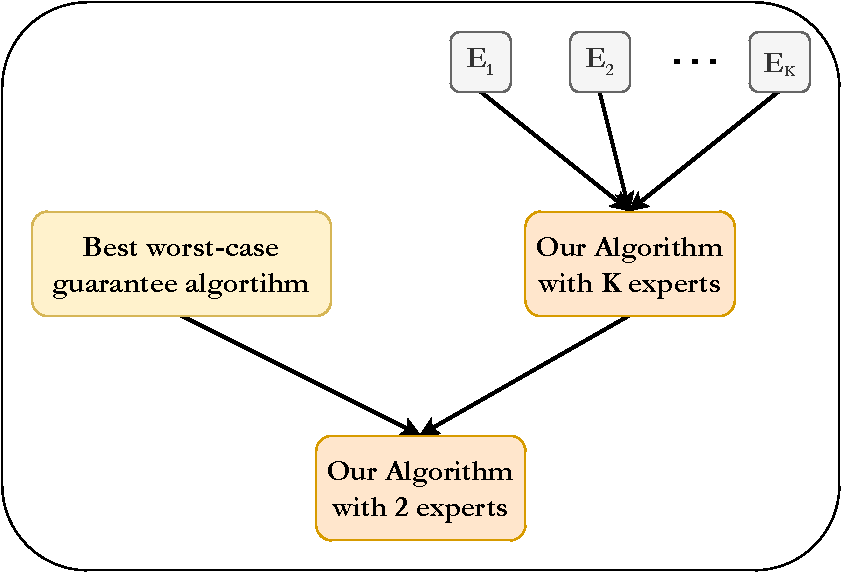
\includegraphics[width=0.4\textwidth]{../paper/Img/algo_structure.pdf}
  \end{center}
  \vspace{-0.5cm}
      \caption{Structural overview of the algorithm's components. $E_1,\ E_2, \dots\ E_K$ correspond to the experts of the online problem.
      On the second layer, we integrate the best standard online algorithm with our algorithm. }
  \label{fig:algo-layers}
   \vspace{-0.8cm}
\end{wrapfigure}

	\noindent If the value of $s_{i,k}^{t}$ is in $\{0,1\}$ for every $i,k,t$, then
	\[
	\rho = \max_{i} \max_{t',t''} \left\{\frac{\sum_{k=1}^{K} s_{i,k}^{t'}}{\sum_{k=1}^{K} s_{i,k}^{t''}} : \sum_{k=1}^{K} s_{i,k}^{t''} > 0 \right\}
	\leq \frac{K}{1}
	\]
	Therefore, the competitive ratio of the our algorithm with the \texttt{LIN-COMB} benchmark is $O(\log (K \rho)) = O(\log (K^2))$.

 	To obtain an algorithm that is competitive with both the \texttt{LIN-COMB} and the worst-case benchmarks, we proceed as follows (\cref{fig:algo-layers} serves as an illustration).
	We first apply the main algorithm on the $K$ experts' integer predictions to obtain an online algorithm, named $A$.
	Algorithm $A$ is $O(\ln (K))$-competitive with the \texttt{LIN-COMB} benchmark. Let $B$ be the algorithm with the best worst-case guarantee.
	We then apply the main algorithm one more time on two algorithms, $A$ and $B$. The final algorithm is $O(\ln (2))$-competitive with both $A$ and $B$.
	In other words, its performance is $O(\ln (K))$-competitive with the \texttt{LIN-COMB} benchmark and is up to a constant factor worse than the best guarantee in the worst-case benchmark.

\end{proof}

By \cref{corollary}, given a $0$-$1$ optimization problem, if there are $K$ deterministic online algorithms, then
we can design an algorithm that has a cost at most $O(\log (K))$ times that of the best linear combination of those algorithms at any time.
Similarly, if $K$ given online algorithms are randomized (they output $0$-$1$ solutions with probabilities), then our algorithm
has an expected cost (randomization over the product of the distributions of those solutions) at most $O(\log(K))$ times that of
the best linear combination of those algorithms at any time. Many practical problems admit $0$-$1$ solutions, for which our algorithm is of interest.
Consider problems like network design, ski rental, TCP acknowledgement, facility location, and so on. Given the fractional solution of our algorithm,
we can apply existing online rounding schemes to obtain integral solutions for such problems.
